\documentclass[12pt,a4paper]{article}

\usepackage[utf8]{inputenc}
\usepackage[T1]{fontenc}
\usepackage[brazil]{babel}
\usepackage{times}
\usepackage{geometry}
\usepackage{graphicx}
\usepackage{booktabs}
\usepackage{float}
\usepackage{caption}
\usepackage{fvextra}

\geometry{left=3cm,right=3cm,top=3cm,bottom=2.5cm}
\captionsetup{font=small,labelfont=bf}
\setlength{\parindent}{1.25cm}
\setlength{\parskip}{0pt}
\emergencystretch=2em

\begin{document}

\begin{center}
{\Large\bfseries Relat\'orio da Atividade 2 -- Etapa 5\\
Detec\c{c}\~ao de Intrus\~oes em Rede CAN\par}
\vspace{0.7cm}

{\normalsize
\'Alvaro C. Negromonte\textsuperscript{1},
Victoria Pessoa Barbosa Matos\textsuperscript{1}\\
Pedro C. Guimar\~aes Rodrigues\textsuperscript{1}\par}
\vspace{0.25cm}

{\normalsize
\textsuperscript{1}Centro de Inform\'atica -- Universidade Federal de Pernambuco (CIn/UFPE)\\
IF747 -- Redes Automotivas -- 2026.1\\
Recife -- PE -- Brasil\\
\texttt{[acn3, vpbm, pcgr]@cin.ufpe.br}\par}
\end{center}

\vspace{0.5cm}

\noindent\textbf{Resumo.}
Este relat\'orio apresenta a avalia\c{c}\~ao do m\'odulo de detec\c{c}\~ao de intrus\~oes
\texttt{id\_time} no ambiente Yes, CARLA CAN. Foram comparadas duas vers\~oes do
detector: a vers\~ao original, que apresentou falsos positivos no cen\'ario normal, e a
vers\~ao melhorada, que normaliza IDs CAN e calcula anomalias sobre intervalos entre
mensagens. Nos logs capturados, a vers\~ao melhorada reduziu os falsos positivos para
zero e detectou 527 intrus\~oes no ID \texttt{0x604} durante o ataque de
\textit{spoofing} do freio de m\~ao.

\section{Introdu\c{c}\~ao}

A Etapa 5 tem como objetivo executar um mecanismo de detec\c{c}\~ao de intrus\~oes em
paralelo com um dos ataques realizados anteriormente e avaliar sua efic\'acia. Para
isso, foi utilizado o detector \texttt{id\_time}, que compara o comportamento temporal das
mensagens CAN recebidas com estat\'isticas de refer\^encia previamente calculadas.

O ataque escolhido para a avalia\c{c}\~ao foi o \textit{spoofing} da fun\c{c}\~ao
\texttt{hand\_brake}. Essa escolha foi feita porque, nas etapas anteriores, esse ataque
teve impacto veicular claro no CARLA e tamb\'em produziu altera\c{c}\~ao quantitativa
expressiva no tr\'afego do ID \texttt{0x604}.

\section{Configura\c{c}\~ao Experimental}

O ambiente foi executado com o DBC padr\~ao \texttt{data/carla.dbc}, mantendo a
compatibilidade com os IDs usados pelo m\'odulo de ataques. O ambiente foi inicializado
com:

\begin{center}
\begin{minipage}{0.92\linewidth}
\begin{Verbatim}[fontsize=\footnotesize,breaklines=true,breakanywhere=true]
./1_up_environment.sh --dbc data/carla.dbc
\end{Verbatim}
\end{minipage}
\end{center}

Em seguida, foram capturados dois logs: um cen\'ario normal, sem ataque, e um cen\'ario
com ataque de freio de m\~ao. A captura do cen\'ario normal foi feita com:

\begin{center}
\begin{minipage}{0.92\linewidth}
\begin{Verbatim}[fontsize=\footnotesize,breaklines=true,breakanywhere=true]
candump -L vcan0 | tee logs/etapa5_normal.log
\end{Verbatim}
\end{minipage}
\end{center}

No cen\'ario de ataque, o IDS foi executado em paralelo com o ataque:

\begin{center}
\begin{minipage}{0.92\linewidth}
\begin{Verbatim}[fontsize=\footnotesize,breaklines=true,breakanywhere=true]
conda run --no-capture-output -n n4s_env python3 intrusion_detection_module.py \
  --detector id_time
\end{Verbatim}
\end{minipage}
\end{center}

\begin{center}
\begin{minipage}{0.92\linewidth}
\begin{Verbatim}[fontsize=\footnotesize,breaklines=true,breakanywhere=true]
conda run --no-capture-output -n n4s_env python3 cyberattacks_module.py \
  --feature hand_brake \
  --period 0.05
\end{Verbatim}
\end{minipage}
\end{center}

Para reproduzir a an\'alise de forma offline, foi utilizado o script de avalia\c{c}\~ao
inclu\'ido no diret\'orio \texttt{data}:

\begin{center}
\begin{minipage}{0.92\linewidth}
\begin{Verbatim}[fontsize=\footnotesize,breaklines=true,breakanywhere=true]
conda run --no-capture-output -n n4s_env python data/id_time_detection_analyzer.py \
  --normal logs/etapa5_normal.log \
  --attack logs/etapa5_handbrake_attack.log \
  --output-dir data/etapa5_detection \
  --plots \
  --compare-versions
\end{Verbatim}
\end{minipage}
\end{center}

\section{Ajuste no Detector}

Durante a prepara\c{c}\~ao da Etapa 5, foram identificadas duas inconsist\^encias no
detector original. A primeira estava relacionada ao formato dos IDs CAN: o arquivo de
estat\'isticas usa IDs no formato \texttt{604}, enquanto o detector comparava as
mensagens recebidas com strings no formato \texttt{0x604}. Assim, IDs conhecidos eram
classificados incorretamente como desconhecidos.

A segunda inconsist\^encia estava na vari\'avel usada para a an\'alise temporal. O
baseline descreve os intervalos entre mensagens, mas o detector calculava estat\'istica
sobre timestamps absolutos. Isso n\~ao representa corretamente o per\'iodo de chegada das
mensagens CAN.

O detector foi ajustado para normalizar os IDs CAN e calcular a m\'edia e o desvio
padr\~ao dos intervalos entre mensagens recentes. Um alerta \'e emitido quando a m\'edia
ou a variabilidade observada se afastam do baseline. Essa altera\c{c}\~ao mant\'em a
proposta original do algoritmo \texttt{id\_time}, mas faz a compara\c{c}\~ao sobre a
m\'etrica correta.

\section{Resultados}

A Tabela~\ref{tab:comparison} resume a compara\c{c}\~ao entre a vers\~ao original e a
vers\~ao melhorada do detector.

\begin{table}[H]
\centering
\caption{Compara\c{c}\~ao entre a vers\~ao original e a vers\~ao melhorada do detector.}
\label{tab:comparison}
\begin{tabular}{lrrl}
\toprule
\textbf{Vers\~ao} & \textbf{Normal} & \textbf{Ataque} & \textbf{Principal ID} \\
\midrule
Original & 2818 & 3026 & V\'arios IDs \\
Melhorada & 0 & 527 & \texttt{0x604} \\
\bottomrule
\end{tabular}
\end{table}

Na vers\~ao original, o detector gerou 2818 alertas no cen\'ario normal. Como esse
cen\'ario n\~ao continha ataque, esses alertas correspondem a falsos positivos. A taxa
observada foi:

\begin{equation}
\frac{2818}{2818} = 100\%
\end{equation}

Ap\'os a melhoria, o detector n\~ao gerou alertas no cen\'ario normal:

\begin{equation}
\frac{0}{2818} = 0\%
\end{equation}

Durante o ataque, a vers\~ao melhorada detectou 527 intrus\~oes no ID \texttt{0x604}.
Esse resultado \'e coerente com o comportamento esperado, pois o ataque injeta mensagens
do freio de m\~ao com per\'iodo de 0,05 s, menor que o per\'iodo normal observado para
esse ID.

\begin{figure}[H]
\centering
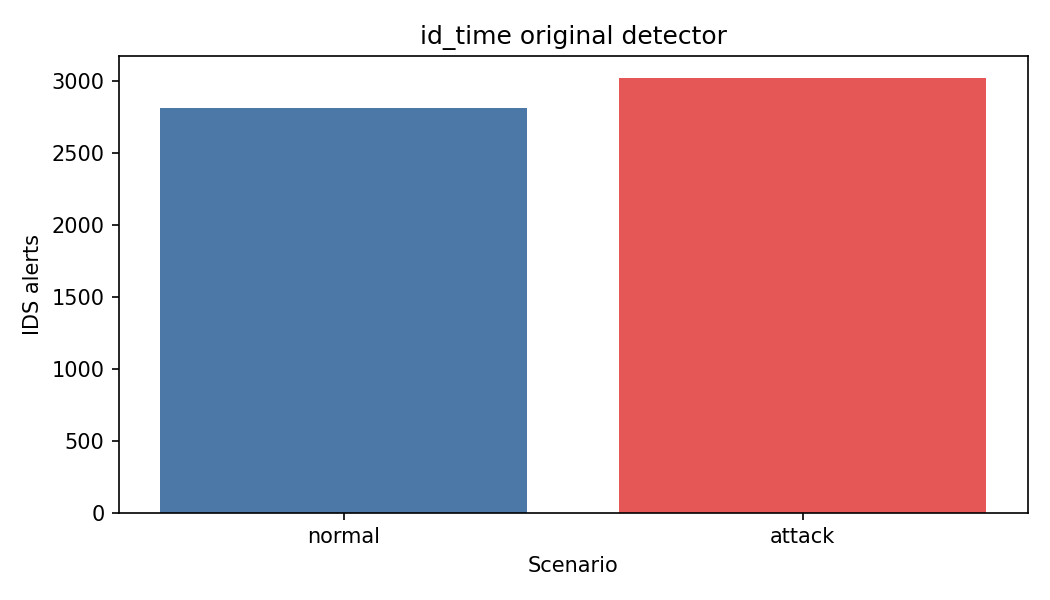
\includegraphics[width=0.82\linewidth]{figures/id_time_detection_counts_original.png}
\caption{Alertas da vers\~ao original do detector nos cen\'arios normal e com ataque.}
\label{fig:original}
\end{figure}

\begin{figure}[H]
\centering
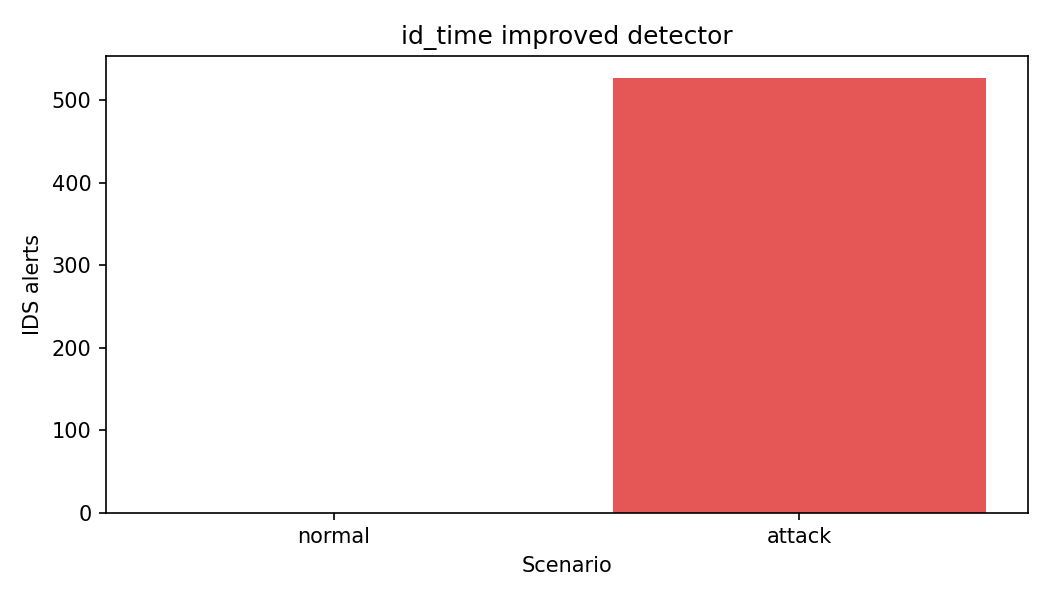
\includegraphics[width=0.82\linewidth]{figures/id_time_detection_counts_improved.png}
\caption{Alertas da vers\~ao melhorada do detector nos cen\'arios normal e com ataque.}
\label{fig:improved}
\end{figure}

\section{Discuss\~ao}

Os resultados mostram que a vers\~ao original do detector n\~ao era adequada para avaliar
o cen\'ario experimental, pois gerava falsos positivos mesmo na aus\^encia de ataques.
O principal motivo era a incompatibilidade de representa\c{c}\~ao dos IDs CAN. Como o
baseline armazenava IDs como \texttt{604} e o detector recebia IDs como \texttt{0x604},
mensagens leg\'itimas eram tratadas como desconhecidas.

Na vers\~ao melhorada, a normaliza\c{c}\~ao dos IDs eliminou esse problema. Al\'em disso,
o c\'alculo temporal passou a usar intervalos entre mensagens, e n\~ao timestamps
absolutos. Com isso, o tr\'afego normal deixou de ser classificado como intrus\~ao,
enquanto o ataque de \textit{spoofing} do freio de m\~ao continuou sendo detectado no
ID correto.

O resultado tamb\'em mostra uma limita\c{c}\~ao do m\'etodo: ele \'e eficaz quando o ataque
altera a periodicidade das mensagens, mas pode ser insuficiente contra ataques que
preservam o per\'iodo esperado e modificam apenas o payload.

\section{Proposta de Melhoria}

Uma melhoria adicional para o algoritmo seria combinar a detec\c{c}\~ao temporal com
valida\c{c}\~ao sem\^antica baseada no DBC. Al\'em de monitorar m\'edia e desvio do
per\'iodo por ID, o detector poderia validar o payload decodificado e as transi\c{c}\~oes
de estado esperadas para cada fun\c{c}\~ao veicular.

Por exemplo, para o freio de m\~ao, o detector poderia observar n\~ao apenas a
frequ\^encia do ID \texttt{0x604}, mas tamb\'em transi\c{c}\~oes repetidas ou persistentes
para o valor ativo. Para marcha r\'e, poderia validar se a mudan\c{c}a de estado ocorre
de forma compat\'ivel com velocidade, marcha e comandos recentes. Essa combina\c{c}\~ao
reduziria falsos negativos contra ataques que imitam o per\'iodo normal, mas alteram o
conte\'udo da mensagem.

Tamb\'em seria recomend\'avel registrar os alertas em CSV ou JSON durante a execu\c{c}\~ao
ao vivo, incluindo timestamp, ID, tipo de alerta e valor observado. Isso facilitaria a
auditoria dos experimentos e a gera\c{c}\~ao autom\'atica de gr\'aficos para relat\'orios.

\section{Conclus\~ao}

A Etapa 5 demonstrou a import\^ancia de validar o pr\'oprio detector antes de avaliar
ataques. A vers\~ao original apresentou falsos positivos no cen\'ario normal, enquanto a
vers\~ao melhorada reduziu a taxa de falsos positivos para zero e manteve a detec\c{c}\~ao
do ataque \texttt{hand\_brake} no ID \texttt{0x604}. Os resultados indicam que a
detec\c{c}\~ao temporal \'e \'util contra ataques que alteram a frequ\^encia das mensagens,
mas deve ser combinada com valida\c{c}\~ao de payload e regras de estado para cobrir
ataques mais discretos.

\end{document}
